\documentclass{nsfc}

\begin{document}

\begin{center}
    \Large\kaishu\textbf{报告正文}
\end{center}

\begin{onehalfspace}
    \large\kaishu
    参照以下提纲撰写，要求内容翔实、清晰，层次分明，标题突出。申请书正文原则上不超过30页，鼓励简洁表达。
    {\color{nsfc_blue}\textbf{请勿删除或改动下述提纲标题及括号中的文字。}}
\end{onehalfspace}

\chapter{立项依据}
{\large\kaishu\color{nsfc_blue}（为什么要开展此项研究，研究的科学技术价值如何）}


\section{研究背景与意义}

研究意义、国内外研究现状及发展动态分析，需结合科学研究发展趋势来论述科学意义；或结合国民经济和社会发展中迫切需要解决\textbf{关键科技问题}（\textbf{Key} Scientific Problems）来论述其应用前景。附主要参考文献目录。

{\kaishu 研究意义、国内外研究现状及发展动态分析，需结合科学研究发展趋势来论述科学意义；或结合国民经济和社会发展中迫切需要解决的关键科技问题来论述其应用前景\cite{latex2e,latex:companion}。附主要参考文献目录。}

如图~\ref{fig:test}~和公式~\eqref{eq:1}~所示。

\begin{figure}[h]
    \centering
    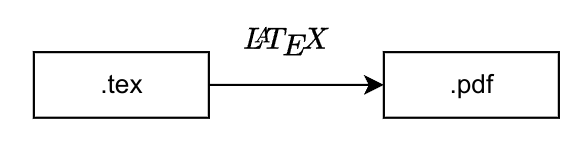
\includegraphics[width=0.4\linewidth]{figure1.png}
    \caption{示例图片}
    \label{fig:test}
\end{figure}

\begin{equation}\label{eq:1}
    f(x) = \int_{-\infty}^\infty  \hat f(x)\xi\,e^{2 \pi i \xi x}  \,\mathrm{d}\xi 
\end{equation}

\subsection{测试测试Testing}

\begin{enumerate}[1.]
    \item 需结合科学研究发展趋势来论述科学意义；
    \item 或结合国民经济和社会发展中迫切需要解决的关键科技问题
    \item 来论述其应用前景。
\end{enumerate}

\bibliography{references}



\chapter{研究内容}
{\large\kaishu\color{nsfc_blue}（提纲不做限制，请按照研究工作的自身逻辑撰写。应提炼出特色与创新点、年度研究计划）}


\chapter{研究基础}

\ctexset{% 利用ctex设置章节样式
    section/format={\zhkai\enkai\color{nsfc_blue}\fontsize{14pt}{16pt}\selectfont},
    section/indent=2em,% 首行缩进
    section/hang=false,% 取消悬挂缩进
    section/aftername={. }, % 编号与标题内容之间
}

\section{\textbf{研究基础与可行性分析}（与本项目相关的研究工作积累和已取得的研究工作成绩，研究风险的应对措施等）;}

无。

\section{\textbf{工作条件}（包括已具备的实验条件，尚缺少的实验条件和拟解决的途径，包括利用国家实验室、全国重点实验室和部门重点实验室等研究基地的计划与落实情况）；}

无。

\section{\textbf{正在承担的与本项目相关的科研项目情况}（申请人正在承担的与本项目相关的科研项目情况，包括国家自然科学基金的项目和国家其他科技计划项目，要注明项目的资助机构、项目类别、批准号、项目名称、获资助金额、起止年月、与本项目的关系及负责的内容等）；}

无。

\section{\textbf{完成国家自然科学基金项目情况}（对申请人负责的前一个已资助期满的科学基金项目（项目名称及批准号）完成情况、后续研究进展及与本申请项目的关系加以详细说明。另附该项目的研究工作总结摘要（限500字）和相关成果详细目录）。}

无。

\chapter{其他需要说明的情况}

\section{申请人同年申请不同类型的国家自然科学基金项目情况（列明同年申请的其他项目的项目类型、项目名称信息，并说明与本项目之间的区别与联系；已收到自然科学基金委不予受理或不予资助决定的，无需列出）。}

无。

\section{具有高级专业技术职务（职称）的申请人是否存在同年申请或者参与申请国家自然科学基金项目的单位不一致的情况；如存在上述情况，列明所涉及人员的姓名，申请或参与申请的其他项目的项目类型、项目名称、单位名称、上述人员在该项目中是申请人还是参与者，并说明单位不一致原因。}

无。

\section{具有高级专业技术职务（职称）的申请人是否存在与正在承担的国家自然科学基金项目的单位不一致的情况；如存在上述情况，列明所涉及人员的姓名，正在承担项目的批准号、项目类型、项目名称、单位名称、起止年月，并说明单位不一致原因。}

无。

\section{同年以不同专业技术职务（职称）申请或参与申请科学基金项目的情况（应详细说明原因）。}

无。

\section{申请人在撰写本申请书时使用生成式人工智能的情况，请详细说明申请书中使用的位置和内容。}

无。

\section{其他（包括但不限于使用以他人名义申报过的申请书；如有，请详细说明）。}

无。

\end{document}
